\section{Model System for the Precision Agriculture System}

\begin{figure}[h!]

	\centering

 	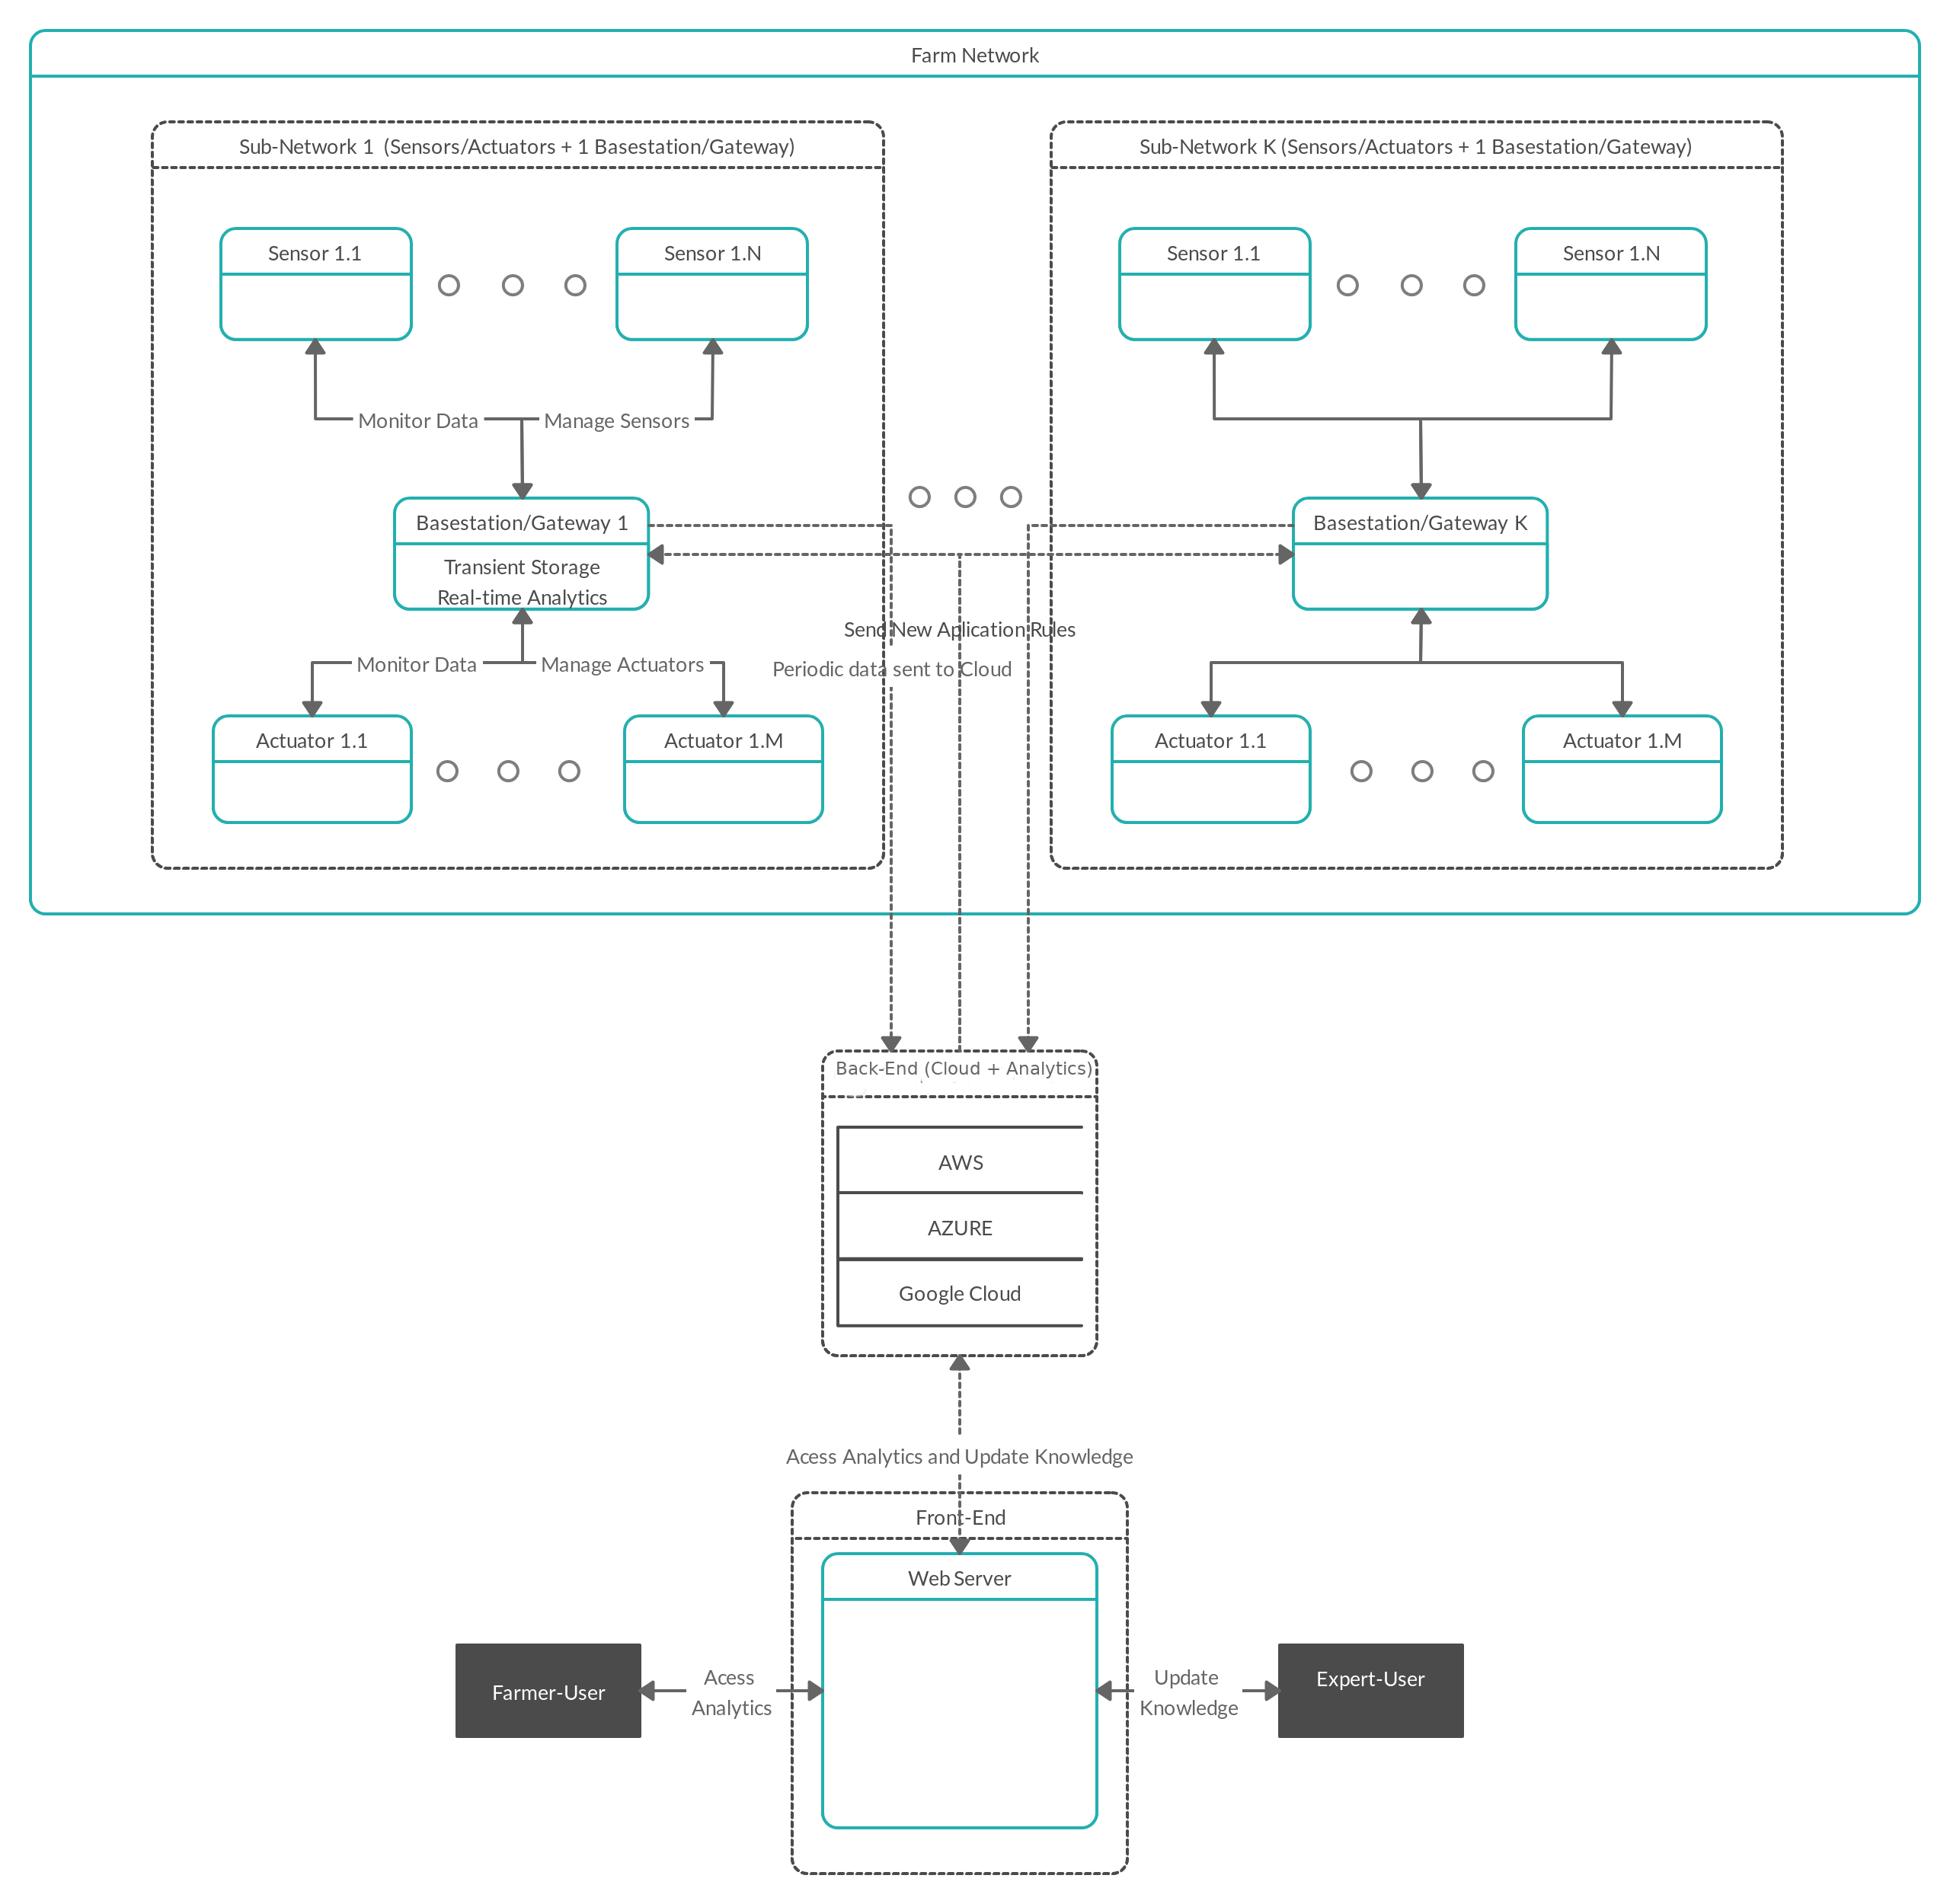
\includegraphics[scale = 0.15]{precisionAgricultureSystem.png}

 	\caption {Model System for the Precision Agriculture System}

  	\label{fig01}
\end{figure}

	O sistema encontra-se dividido em três boundaries principais a cloud, o sistema de agricultura e o front-end.Ainda dentro da boundary do sistema de agricultura divide-se em pequenos sub-sistemas que correposndem ao conjunto de uma basestation/gateway junto com os sensores e actuators.

	A partir do modelo entende-se que os sub-sistemas referidos anteriormente não comunicam entre si, só com a cloud , de forma a atualizar as configurações das basestations/Gateways.Também o back-end, formado pelo armazenamento em cloud e o modulo de analytics, p'só deve comunicar com as basestations/gateways e com o servidor do front-end fornecendo uma API para comunicar com o mesmo.Finalmente, temos o front-end que para além da Cloud so comunica com dois tipos de utilizadores externos ao sistema que são os agricultores e os Experts.

	É importante salientar que o back-end deste sistema está usando alguns dos forncedores indicados na figura , o que , por si só, já fornece algumas garantias de segurança para a proprio sistema de armazenamento.Na seção seguinte analisar-se-á mais detalhadamente cada parte deste sistema de forma a encontrar possíveis ameaças subjacentes a essas boundaries e elementos.

	Nas duas seguintes imagens encontra-se se generalizados os dois processos principais executados pelos dois tipos de utilizadores.Apesar de encontrar-se representado o acesso aos dados pelo Farmer, é esperado que o Expert tambem requisite-os.No entanto, só o Expert é que irá alterar os dados da base dados para melhor o knowledge do sistema.

\begin{figure}[h!]

	\centering

 	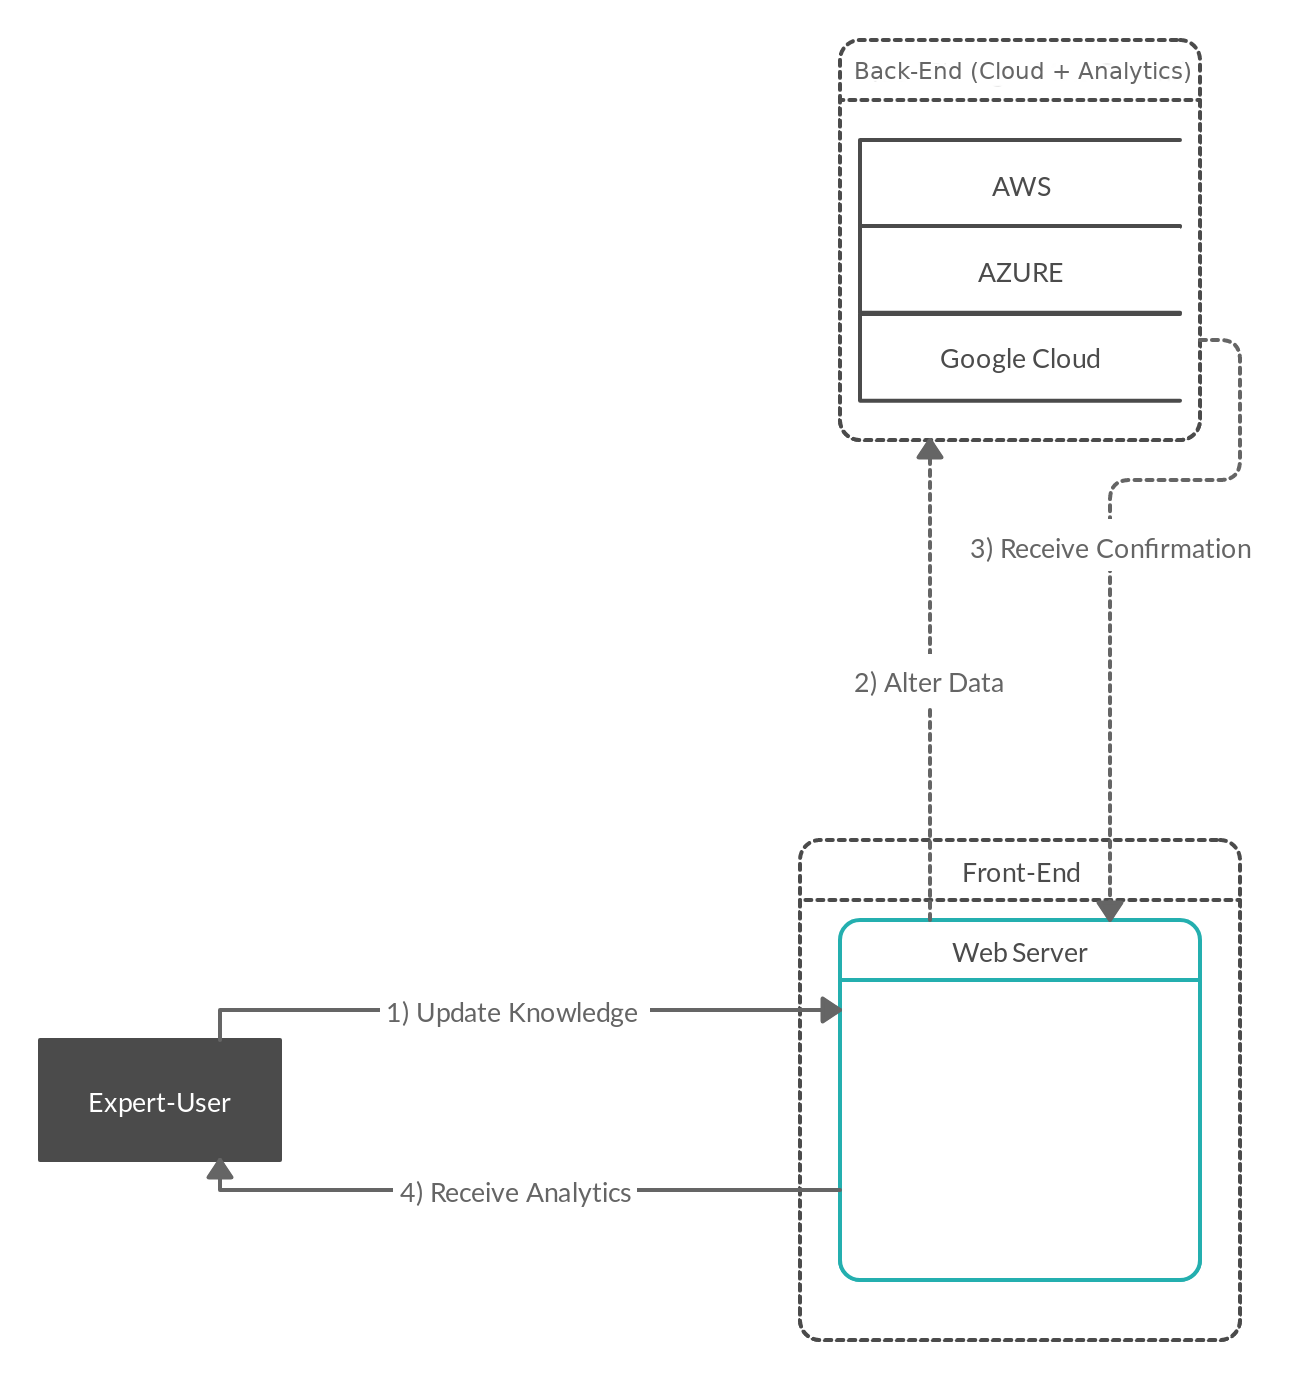
\includegraphics[scale = 0.15]{ExpertAlter.png}

 	\caption {Uploading Data by Expert}

  	\label{fig02}
\end{figure}



\begin{figure}[h!]

	\centering

 	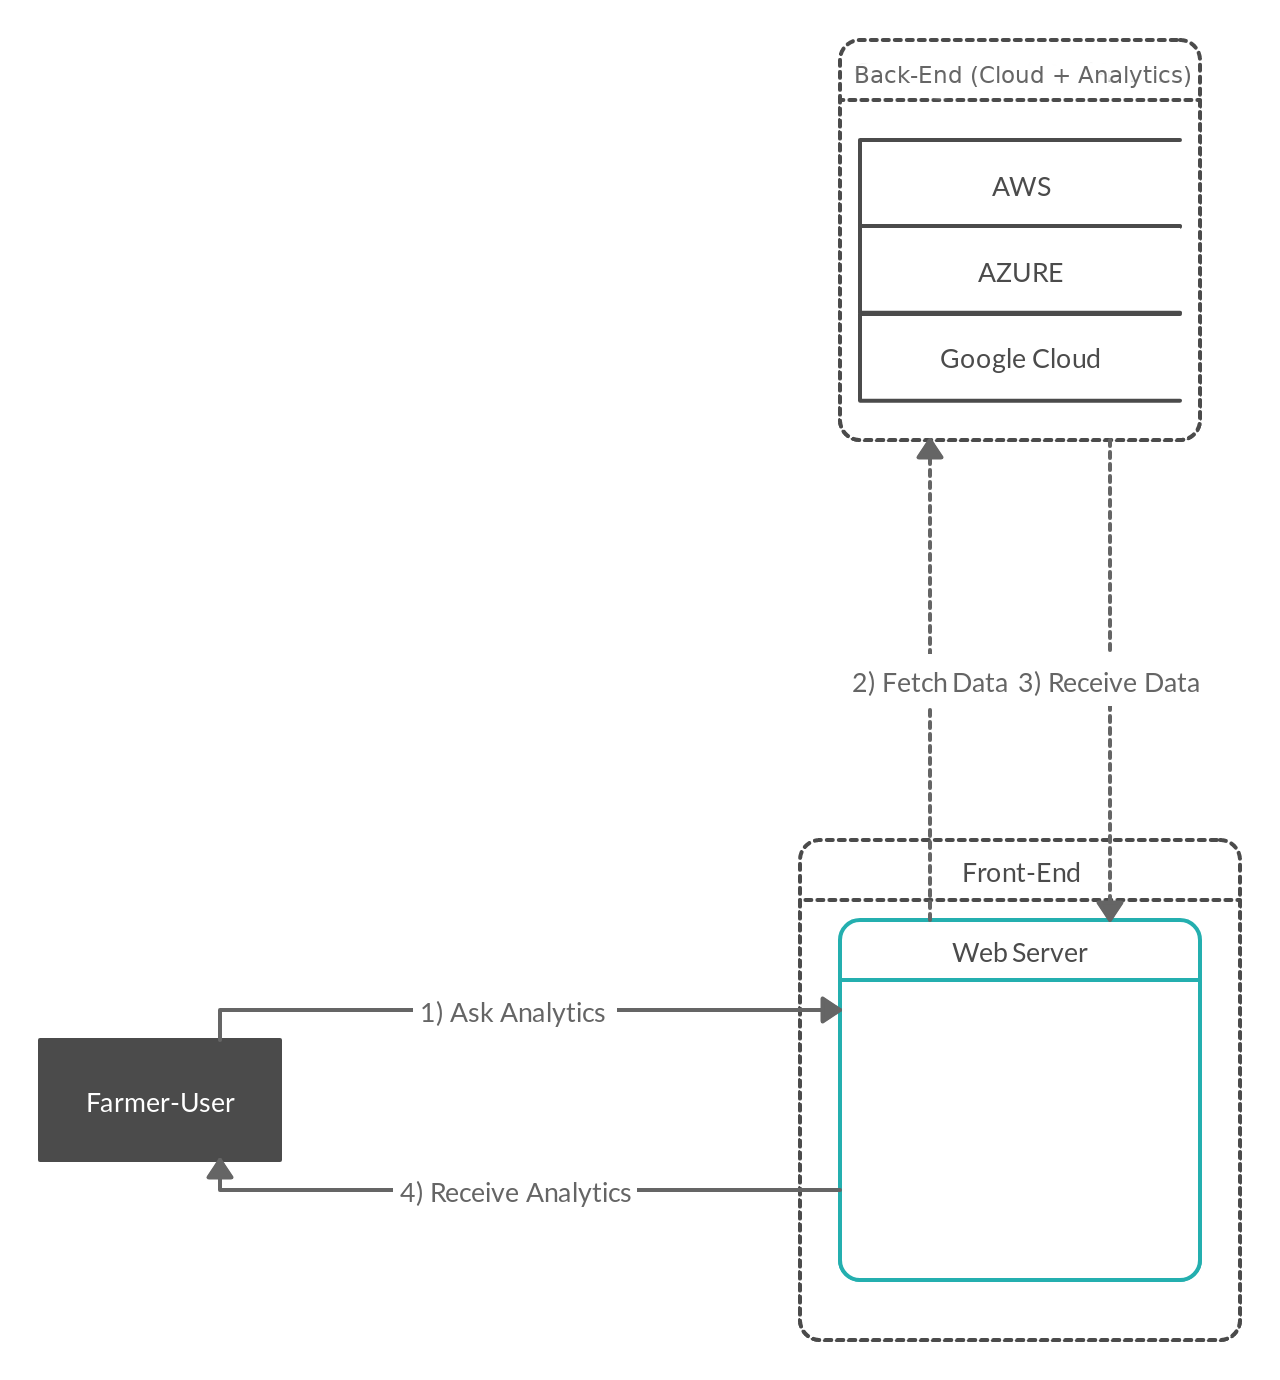
\includegraphics[scale = 0.15]{FarmerAcess.png}

 	\caption {Acessing Data by Farmer}

  	\label{fig03}
\end{figure}

% Meter a parte que falta aqui da farm

\section{Finding \& Addressing Threats}

	De forma a encontrar as ameaças referentes ao sistema ir-se-á analisar cada elemento seguindo STRIDE.Cada subseção corresponde a um dos três subsistemas definidos anteriormente.



\subsection{FrontEnd}

\subsubsection{Spoofing}
\label{Spoofing}
\hfill\\
\begin{itemize}

\item Um atacante poderia conetar ao sistema em 1) e 3) em  na figura \ref{fig02} ou em \ref{fig03} caso este nao tenha nenhum sistema de autentificação tanto para os utilizadores do Front-end como para o Front-end em si ao conetar-se ao Back-End.Para mitigar esta ameaça é necessário tanto um sistema de autentificação para os utilizadores (login) como um sistema para gerenciar as sessões do mesmo(Encrypted cookies,Session Keys).Enquanto na ligação do Front-End ao Back-End é tambem necessário alguma forma de Autentificação(Tickets Kerberos,IPsec). Assim, so permitir-se-ia só ao servidores Front-End autorizados aceder a API do Back-End e solicitar dados do mesmo.

\hfill\\
\item Um atacante em 1) poderia tentar fazer login na aplicaçao front-end como farmer/Expert através de tentativas sucessivas de pares user/password.De forma a mitigar o problema poderia-se implementar delay quando o sistema nota muitas tentativas de login.Este medida tem consequências visto que pode ser utilizada em contra do sistema.Apesar do atacante não conseguir descobrir os pares login/password caso fosse realizado o mesmo ataque passaria a um DoS para os utilizadores do Front-End que nunca poderiam conetar-se.Possivelmente uma Firewall ajudaria a mitigar esta ameaça.

\hfill\\
\item Um atacante poderia criar um "clone" do web-server de forma a enganar o cliente para inserir os dados de login.Assim obtem acesso ao sistema ao nivel do utilizador.A mitigação deste ataque é possível através do uso de credenciais no Front-End que serão guardadas pelo browser do utilizador. 

\hfill\\
\item Um atacante irá sempre utilizador o método com a segurança mais fraca, como consequência dever-se-á obrigar sempre as ligações com protocolos com encriptaçao(HTTPS/IPsec)

\end{itemize}

\subsubsection{Tampering}
\hfill\\
\begin{itemize}

\item Um atacante poderia enviar dados modificados/alterar dados referentes ao sensores em 4) na figura \ref{fig02} de forma a enganar o cliente sobre o estado dos sensores e da quinta.Utilizando um mecanismo de encriptação e de Integradade(HTTPS) na comunicação dos dados este ataque pode ser mitigado.

\end{itemize}

\subsubsection{Repudiation}
\hfill\\
\begin{itemize}

\item Um utilizador do tipo Expert poderia em 1) na figura \ref{fig03} mandar um pedido para alterar a knowledge do sistema de forma a piora-lo e não admitir essa alteraçao.Para evitar esta situação poderia manter Logs de alterações feito pelos Experts no armazenamento na Cloud.

\end{itemize}

\subsubsection{Information Disclosure}
\hfill\\
\begin{itemize}
\item Admitindo que a aplicação pode dar suporte a diferentes farms. Um utilizador ja loggado pertence a concorrência poderia pedir acesso a ficheiros da concorrência.Uma fácil solução será implementar ACLs para restringir acesso aos ficheiros ou na logica do aplicação WEB do Front-End.

\hfill\\

\item Outros problemas como man-in-middle, acesso ao ficheiro não encriptado,etc. Sao resolvidos com alguns do métodos referidos anteriormente.
\end{itemize}

\subsubsection{Denial of Service}
\hfill\\
\begin{itemize}

\item Como referido em \ref{Spoofing} no primeiro ponto sobre Spoofing, poderia causar DoS usando o delay para prevenir tentativas de brute force das passwords.

\hfill\\
\item Um atacante depois de entrar no sistema Front-End como Expert podendo tentar atualizar o sistema atraves de vários PCs com login na mesma conta.Provocando que o Servidor não conseguisse satisfazer todos os pedidos.O mesmo poderia ser feito caso fosse feito login como Farmer atraves de varios GETs.O Profiling do tráfego da rede como anomalias e reputações de IP mitigariam o ataque.

\end{itemize}

\subsubsection{Elevation of Privilege}
\hfill\\

\begin{itemize}

\item

\end{itemize}

